\chapter{Design}
In this chapter, we dwell into the detailed design of the project. Section~\ref{sec:module} lists the individual modules designed in this project. Section~\ref{sec:hardware} gets into details of all the hardware design; section~\ref{sec:software} does the same for software design. Finally section~\ref{sec:desIndust} dwells into details of industrial design of the project.
\begin{figure}[H]
\centering
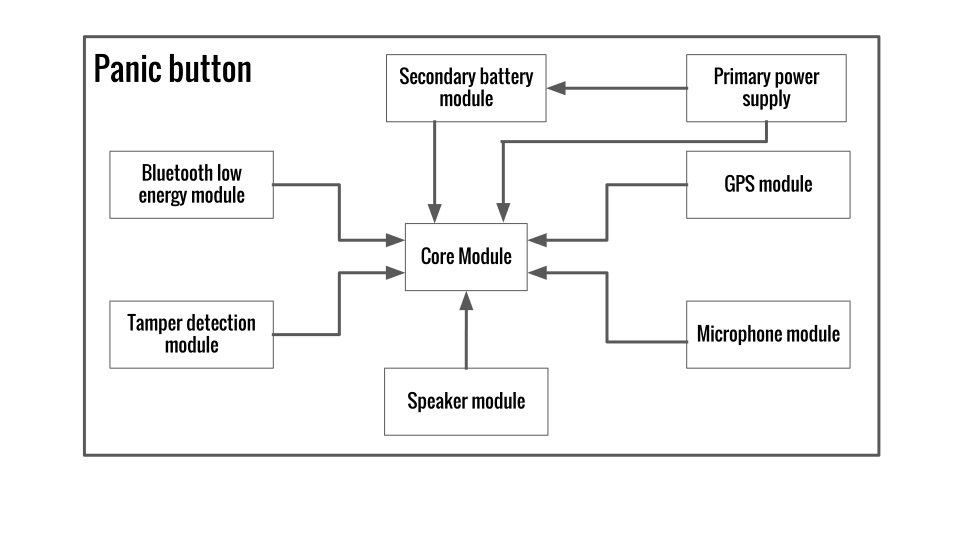
\includegraphics[width=\textwidth]{block_dia}
\caption{Block diagram of the \emph{PanicButton device}}
\label{fig:block_dia}
\end{figure}

%The chapter includes
%\begin{itemize}
%\item design of modules and sub-modules
%\item design equations (with electrical and thermal stresses)
%\item component selection
%\item design of algorithms
%\item industrial design aspects
%\item system integration issues
%\end{itemize}

\section{Module partitioning}
\label{sec:module}
This section gives an overview for the content in next two sections. Section~\ref{sec:hardware} describes the design of hardware used in the project. It is divided in three major sections-
\begin{itemize}
\item \emph{PanicButton device}- describes the design of core module, tamper detection module, etc.
\item Server- describes the hardware involved in server and,
\item Smartphone- describes the hardware involved in smartphone.
\end{itemize}

Section~\ref{sec:software}, describes the design of the firmware used in the project. This section dwell in to the software design aspects of-
\begin{itemize}
\item System validation module,
\item Audio streaming module,
\item Global Positioning System module,
\item Panic button module and,
\item Audio-based trigger module.
\end{itemize}  
 
%Based on the module and sub-module partitioning of the previous chapter
%\begin{itemize}
%\item the segregation of modules into hardware, embedded software and standalone
%software parts
%\item the exhaustive list of stimuli to the modules (hardware and software)
%\item detailed quantification of the stimuli for both hardware and software
%modules
%\end{itemize}

\section{Hardware design}
\label{sec:hardware}
\subsection{\emph{PanicButton device}}
\subsubsection{Core-module}
The core-module for the system is based on Raspberry pi 3. Raspberry pi uses BCM2837 SOC from Broadcom, with four ARM Cortex-A53 64-bit cores running at 1.2GHz, a Broadcom VideoCore IV Graphics Processing Unit (GPU), 1 GB LPDDR2 Random access Memory (RAM) which runs at 900MHz, 10/100 Ethernet, 2.4GHz 802.11n Wireless Fidelity (WiFi) and micro secure digital (microSD) card with maximum size of 128 GB. Peripherals connects to a High-Definition Multimedia Interface (HDMI) port, four Universal Serial Bus (USB) 2.0 ports, one audio-video port, Camera Serial Interface (CSI) and Display Serial Interface (DSI) available on board.
Raspberry pi 3 has a 40-pin Header, which contains one Serial peripheral interface (SPI) with two chip select pins, one Inter-integrated Circuits (I2C), one Universal Asynchronous Receiver Transmitter (UART) and 18 General Purpose Input Output (GPIO) pins.
The schematic of the core-module is shown in figure~\ref{fig:core_module_sch}.
\begin{figure}[H]
\centering
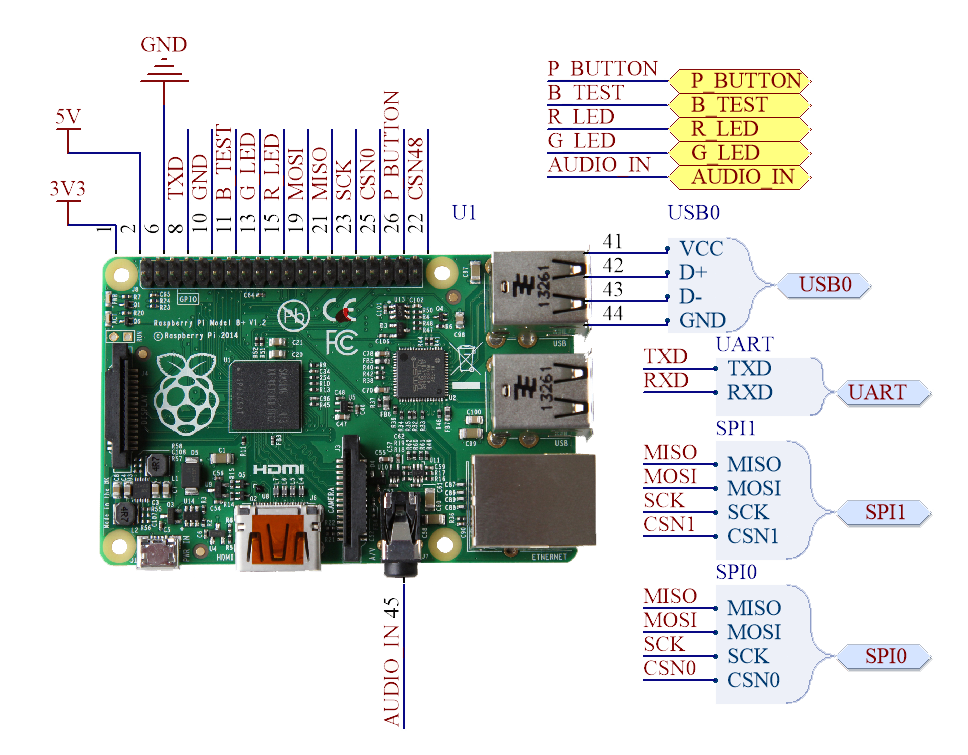
\includegraphics[height=10cm]{core_module_sch}
\caption{Schematic of the core-module of the \emph{PanicButton device}}
\label{fig:core_module_sch}
\end{figure}


\subsubsection{Tamper detection module}
The \emph{PanicButton device} is installed in public transport, which makes it very vulnerable to tampering. In order to tamper with the device, they must first open the enclosure. The tamper detection module detects opening of the lit/top panel by using a switch and stores that information in non-volatile memory. The normally closed type switch is connected between the base of enclosure and the top lid; It changes its state when lid is opened. The tamper detection module uses an ultra lower power MSP430G2553 microcontroller running on CR2032 Lithium ion coin cell auxiliary battery. SPI interface is used to communicate between the microcontroller and the core-module.
\begin{figure}[H]
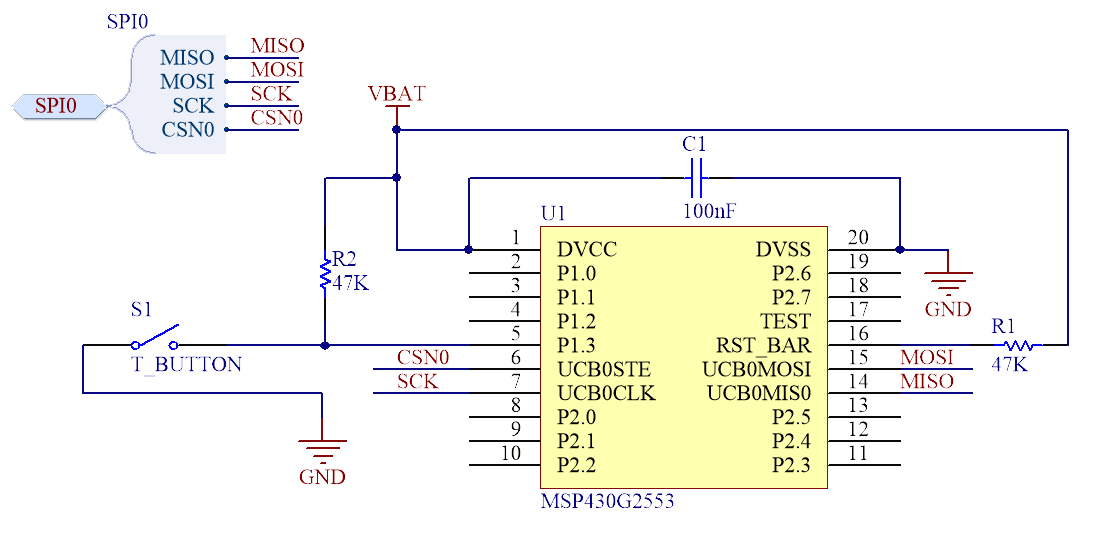
\includegraphics[width=\textwidth]{tamperingproofsytem_sch}
\caption{Schematic of Tamper detection module}
\label{fig:tamperingproofsytem_sch}
\end{figure}

\subsubsection{Panic button \& LED drive module}
Panic button is a normally open non-latching type switch with 10 kOhm pull resistor which pulls it up to 3.3 V. A 2N4401 transistor is used in parallel with the switch to emulate the switch press to test the functioning of the switch. 100 kOhm resistor connected to the base terminal of the transistor, limits the current flowing through the base and emitter terminals. \textit{B\_TEST} is output from core-module and \textit{P\_BUTTON} is input to the core-module.
Two 2N4401 are used to drive four red and four green LEDs for status indication. \textit{R\_LED} and \textit{G\_LED} are output from the core-module to drive these LEDs. The schematic of module is shown in figure~\ref{fig:pbutton_sch}.
\begin{figure}[H]
\begin{subfigure}{.5\textwidth}
  \centering
  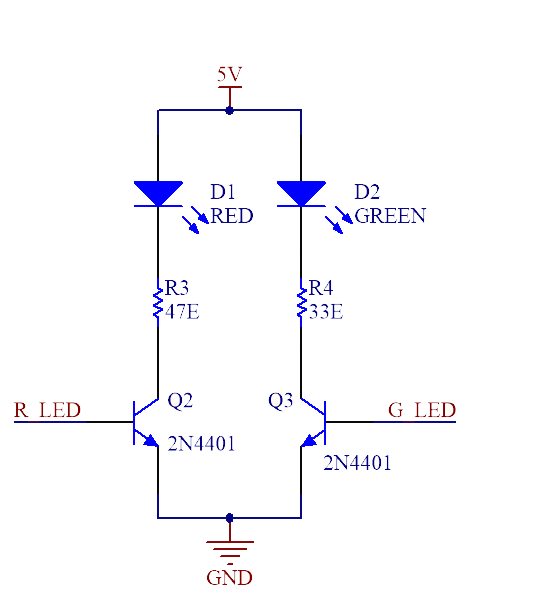
\includegraphics[width=.95\linewidth]{pbutton_sch}
  \caption{}
  \label{fig:p_button_a}
\end{subfigure}%
\begin{subfigure}{.5\textwidth}
  \centering
  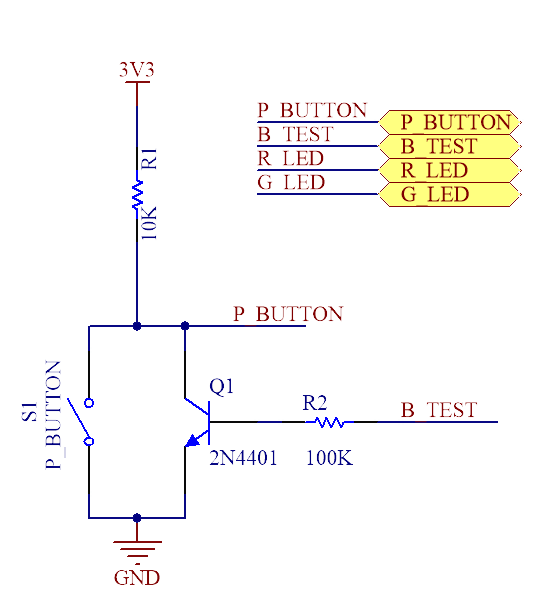
\includegraphics[width=.95\linewidth]{rg_led}
  \caption{}
  \label{fig:p_button_b}
\end{subfigure}
\caption{Schematic of (a) LED driver (b) Panic button}
\label{fig:pbutton_sch}
\end{figure}

\subsubsection{GPS module}
The Global Positioning System (GPS) module is NEO-6M module from Ublox. NEO-6M uses AssistNow Autonomous Technology,  which provides functionality similar to Assisted GPS (A-GPS) without the need of external network connection. Based on previously broadcast satellite ephemeris data downloaded to and stored by the GPS receiver. AssistNow Autonomous Technology generates accurate satellite orbital data(``AssistNow Autonomous data") that is used for the future GPS position fixes. Electrically Erasable Programmable Read-Only Memory (EEPROM) is used to store parametric data of GPS receiver (NEO-6M).
UART protocol is used to connect GPS module to the core-module as shown in figure~\ref{fig:gps_sch}.    % NEO-6M uses aiding information like ephemeris, almanac, rough last position and time and satellite status and an optional time synchronous signal to reduce time to first fix significantly and improve the acquisition sensitivity.
\begin{figure}[H]
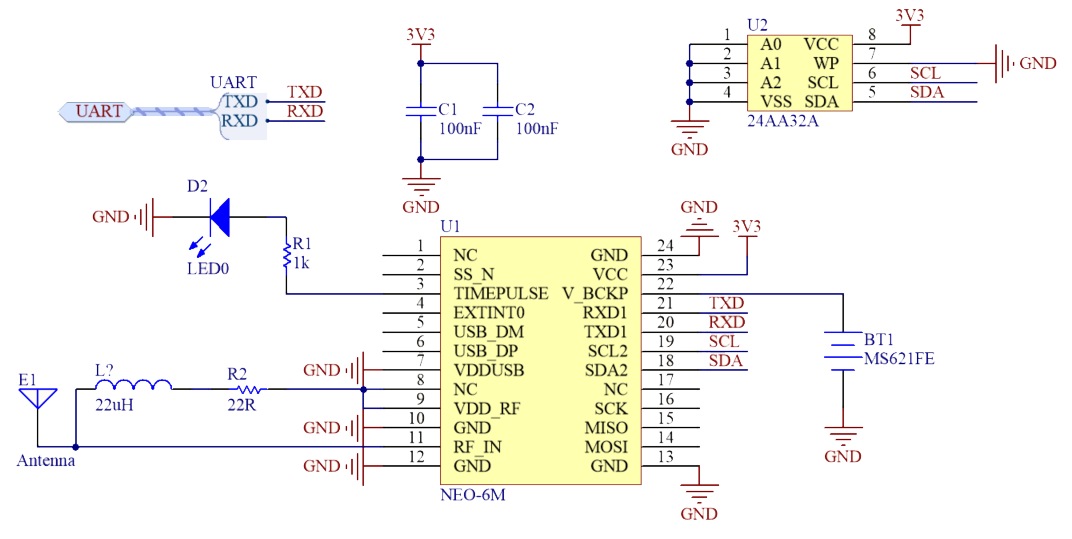
\includegraphics[width=\textwidth]{gps_sch}
\caption{Schematic of GPS module}
\label{fig:gps_sch}
\end{figure}

\subsubsection{Bluetooth low energy module}
The Bluetooth Low Energy (BLE) module uses nRF51822QFAC SOC from Nordic Semiconductors. nRF51822 SOC has ARM\textsuperscript{\textregistered} Cortex\textsuperscript{\texttrademark}-M0 32-bit processor running at 16 MHz with 256 kB of embedded flash program memory and 32 kB of RAM. It requires one crystal for system clock and one 32.768 kHz crystal for real time clock functionality. It uses 50 $\Omega$ impedance matching circuit for maximum radiation as shown in right hand side of figure~\ref{fig:ble_sch}.\\
4-wire SPI interface is used to connect the SOC to the core-module. 
\begin{figure}[H]
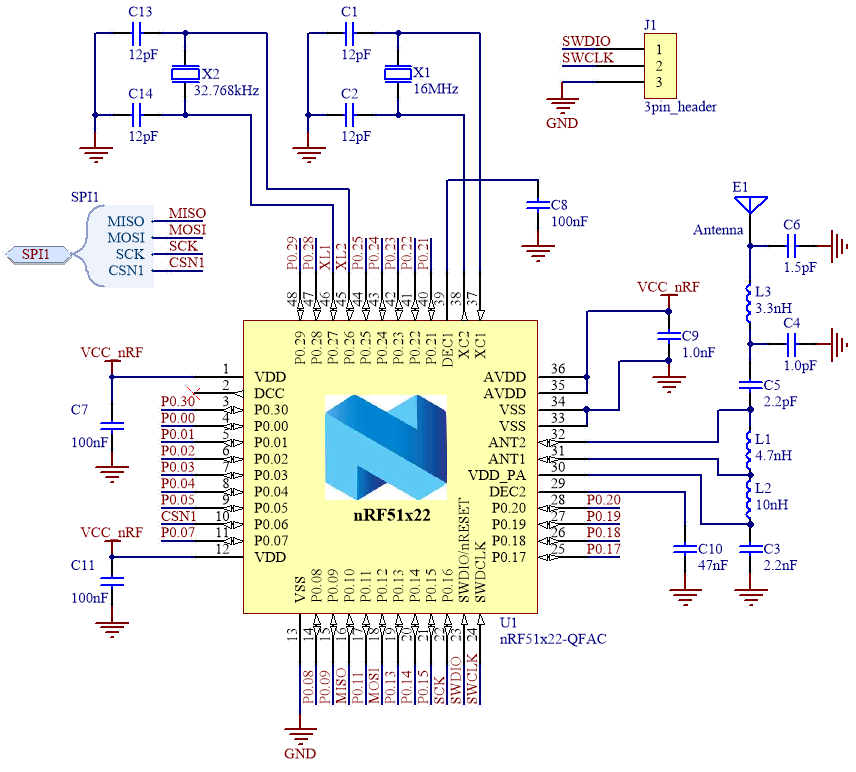
\includegraphics[width=\textwidth]{ble_sch}
\caption{Schematic of Bluetooth low energy module}
\label{fig:ble_sch}
\end{figure}

\subsubsection{Speaker module}
A 8 $\Omega$ 0.5 watt speaker and microphone pair is used to validate the microphone in a closed loop. As core-module cannot drive the 8 $\Omega$ speaker directly, we designed LM386 Integrated Circuit (IC) based amplifier to drive the speaker. A 10 k$\Omega$ potentiometer is used in series with 10 uF bypass capacitor to adjust the gain manually as shown in figure~\ref{fig:speaker_amp_sch}.
\begin{figure}[H]
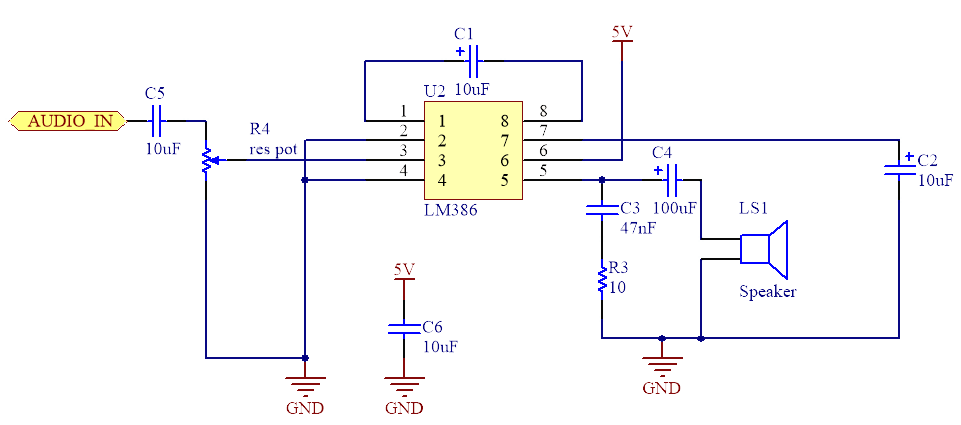
\includegraphics[width=\textwidth]{speaker_amp_sch}
\caption{Schematic of speaker amplifier module schematic}
\label{fig:speaker_amp_sch}
\end{figure}

\subsubsection{Microphone module}
Core-module does not have an on-board audio input support. We used external USB sound-card to add audio input(microphone) to the core-module as shown in the figure~\ref{fig:audio_trigger_sch}.% The sound-card measured 11.2 x 8.4 x 2.1 cm and weighed 82 grams. An omni-directional microphone gets connected at the input port of the sound card. Hardware for audio-based trigger is shown in figure~\ref{fig:audio_trigger_sch}.
\begin{figure}[H]
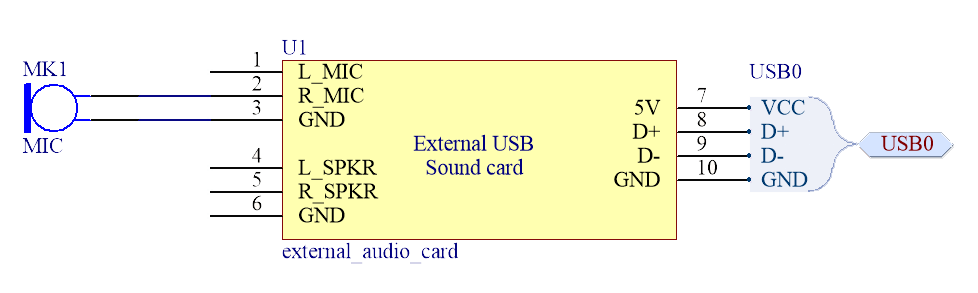
\includegraphics[width=\textwidth]{audio_trigger_sch}
\caption{Schematic for microphone module}
\label{fig:audio_trigger_sch}
\end{figure}

\subsection{Back-end server}
We used a desktop computer as the back-end sever with specification given below.
\begin{itemize}
\item \textbf{Processor:} Intel\textsuperscript{\textregistered} Core\textsuperscript{\texttrademark} i5-4440 quadcore processor running at 3.1 GHz.
\item \textbf{Graphics processor:} Integrated Intel\textsuperscript{\textregistered} HD Graphics 4600 running at 350 MHz.
\item \textbf{RAM:} Kingston value RAM 16 GB DDR3 running at 1600 MHz.
\item \textbf{Hard disk:} Seagate SATA SSHD 1 TB desktop internal hard drive 7200RPM.
\end{itemize}

\subsection{Smartphone}
We used a Google Nexus 4 smartphone running Android 5.1.1 to test designed application. The specification of the smartphone are given below. 
\begin{itemize}
\item \textbf{SOC:} Qualcomm APQ8064 Snapdragon S4 Pro with four Krait running at 1.5 GHz and Adreno 320 GPU running at 400 MHz.
\item \textbf{Radio:} Wi-Fi 802.11 a/b/g/n and Bluetooth v4.0.
\item \textbf{Battery:} 2100 mAh.
\item \textbf{Screen:} 4.7 inches 768 x 1280 pixels In-Plane Switching (IPS) display.
\end{itemize}

\emph{Note: Any smartphone with Bluetooth v4.0 or above and running Android 4.3 or above can be used.}

%Based on the stimuli classification of each module or sub-module,
%perform the design which includes
%\begin{itemize}
%\item the final circuit schematic
%\item design equations relating to functional aspects like accuracy, resolution,
%dynamics and harmonics with respect to the output
%\item design equations relating to electrical stresses of components or
%devices
%\item design equations relating to thermal stresses of components or devices
%\item selection of devices based on the design equations
%\item selection of associated non-electrical parameters and components like
%heat sink, wires, connectors, switches etc.
%\item reliability estimate in terms of mean time to failure (MTTF)
%\end{itemize}
%NOTE: \emph{include as many sections/sub-sections as there are hardware
%modules/sub-modules and repeat the above for every hardware module
%and sub-module}.


\section{Software design}
\label{sec:software}
\subsection{System validation module}
The system validation module is responsible for self checking and notifying the user about the status of the system. The system validation module tests the microphone, panic button, firmware and enclosure tamper state.\\
The microphone and panic button validation runs every time a new user boards the vehicle or a user wants to re-validate the system. The microphone and the panic button has a five second timeout period after which the validation state is invalidated. The firmware validation is done after every reset and it doesn't have a timeout period. The enclosure tamper detection is an always-on validation sequence, which syncs its state every minute with tamper detection hardware.\\   
The flow chart of system validation procedure is shown in figure~\ref{fig:ble_validation}. \\
The components involved in the validation of the system are as follows.
\begin{itemize}
\item User's smartphone
\item nRF51822 BLE SOC
\item Core-module
\item Server
\end{itemize}
User's smartphone connects to the nRF51822 and sends a random \emph{connectionID} to it and closes the connection. User's smartphone waits for the response from the server. The nRF51822 relays the \emph{connectionID} to the core-module. Core-module checks whether the previous validation results are still valid. If it is not valid, then core-module will start the validation sequence to validate the state of the system. If the previous validation results are valid or the current validation sequence completes, then core-module sends the validation results, \emph{connectionID}, \emph{date-time} and encrypted \emph{panicButtonID} to the server. If the server finds the \emph{panicButtonID} in the database, then it sends the driver details, vehicle details and validation results to the user's smartphone. The user's smartphone will show a notification to interrupt the user, which contains the information received from the server.\\
The flowchart of the system validation module is shown in figure~\ref{fig:ble_validation}.
Next we will look into the working of individual components.
\begin{figure}[H]
\centering
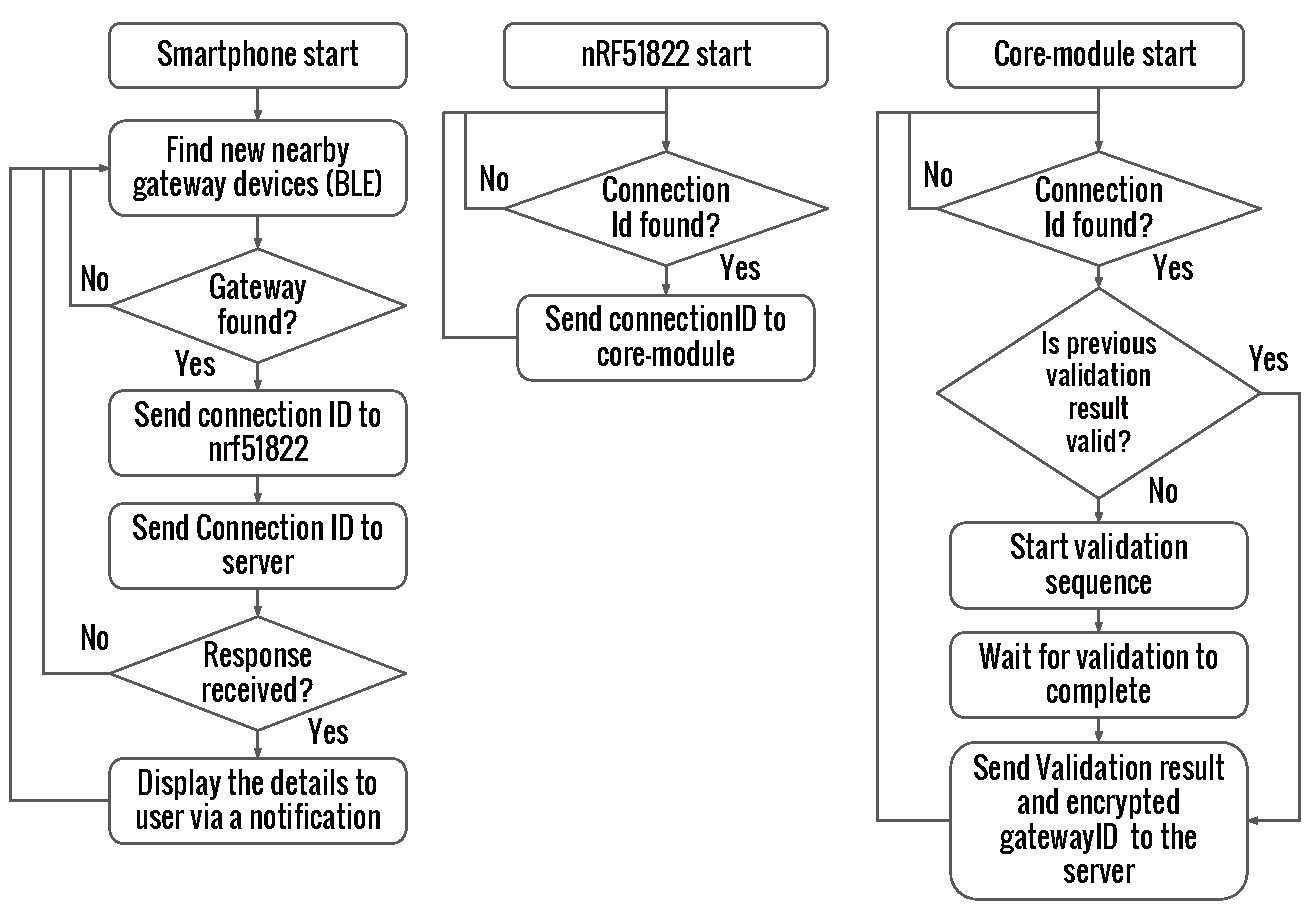
\includegraphics[width=\textwidth]{ble_validation.pdf}
\caption{Flow chart for BLE system validation module}
\label{fig:ble_validation}
\end{figure}
\textbf{nRF51822}
acts as a relay between core-module and user's smartphone. nRF58122 uses Generic Access Profile (GAP) to control the connections and advertising. BLE's GAP layer is responsible to broadcast connectible beacons to show \emph{PanicButton device}'s presence to the nearby devices for them to connect.\\
nRF51822 is running a Generic Attribute Profile (GATT) server to serve the validation service with \emph{connID} characteristic. The UUID used are shown in table~\ref{tab:Ids}.

\begin{table}[H]
\begin{center}
\begin{tabular}{ |c|c| } 
 \hline
 \textbf{} & \textbf{UUID}\\
 \hline 
 \hline
  Validation service & 6E400001-B5A3-F393-E0A9-E50E24DCCA9E\\ 
 \hline
 \emph{ConnID} characteristic & 6E400002-B5A3-F393-E0A9-E50E2DCCA9E \\ 
 \hline
\end{tabular}
\end{center}
\caption{UUIDs of the BLE services} 
\label{tab:Ids}
\end{table}

%\begin{itemize}
%\item \textbf{Validation service} 6E400001-B5A3-F393-E0A9-E50E24DCCA9E
%\item \textbf{\emph{ConnID} characteristic} 6E400002-B5A3-F393-E0A9-E50E2DCCA9E
%\end{itemize}
nRF51822 forwards the \emph{connectionID} received from user's smartphone  to the core-module using SPI protocol.

\textbf{Android app} runs on user's smartphone as a background service to scan for nearby \emph{PanicButton devices}. App differentiates the \emph{PanicButton device} from other devices using services they offer i.e., if some device has the service and characteristics IDs as mentioned in table~\ref{tab:Ids}, it considers the device as a valid \emph{PanicButton device}.\\
As soon as a valid \emph{PanicButton device} is found, the app connects to the \emph{PanicButton device} and sends a pseudo random 32-bit number to it and disconnects. After disconnection from the \emph{PanicButton device}, app sends the same number to the server and waits for server's response. Once the server's response is received, app builds a notification with information received from server and display it to the user. In case the validation of the \emph{PanicButton device} is successful, it will display ``Welcome, safe to enter", otherwise it will display ``Caution, enter at your own risk". The screeshots of the android app is shown in figure~\ref{fig:android_screenshot}. 

\begin{figure}[H]
\begin{subfigure}{.5\textwidth}
  \centering
  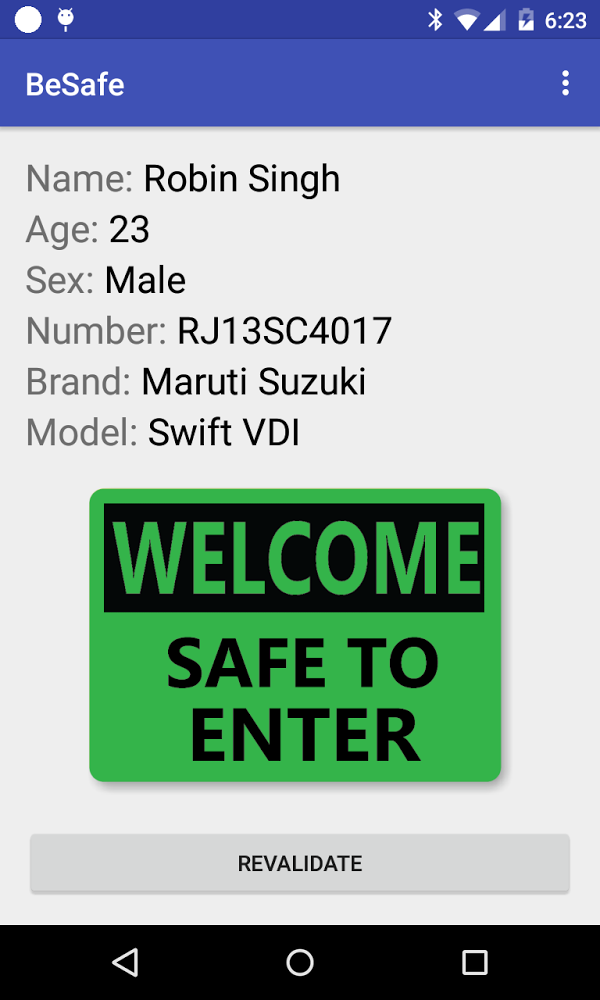
\includegraphics[width=.9\linewidth]{android_safe}
  \caption{Screenshot of ``Welcome, safe to enter"}
  \label{fig:android_safe}
\end{subfigure}%
\begin{subfigure}{.5\textwidth}
  \centering
  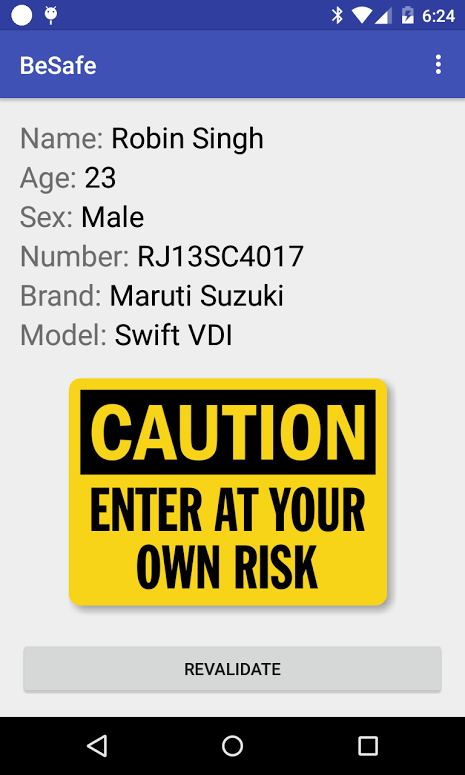
\includegraphics[width=.9\linewidth]{android_caution}
  \caption{Screenshot of ``Caution, enter at your own risk"}
  \label{fig:android_caution}
\end{subfigure}
\caption{Screenshots of Android app}
\label{fig:android_screenshot}
\end{figure}



\textbf{Core-module} receives \emph{connectionID}, when a user's smartphone connects to nRF51822. The core-module will add the \emph{connectionID} to the queue of \emph{connectionIDs}. Each \emph{PanicButton device} has it own unique and secret 128-bit  \emph{panicButtonID} stored in the core-module associated with it, embedded in the non-volatile memory. The \emph{panicButtonID} is used to validate the identity of the \emph{PanicButton device} to the server.
After receving the \emph{connectionID} for the user's smartphone, the core-module will start a new validation sequence if the previous validation result is not valid anymore due to timeout event. Once a valid validation result is ready, the core-module will merge \emph{connectionID} and \emph{panicButtonID} into \emph{mergedID}. The data flow for merging the IDs is shown in figure~\ref{fig:merged_id}.
\begin{figure}[H]
\centering
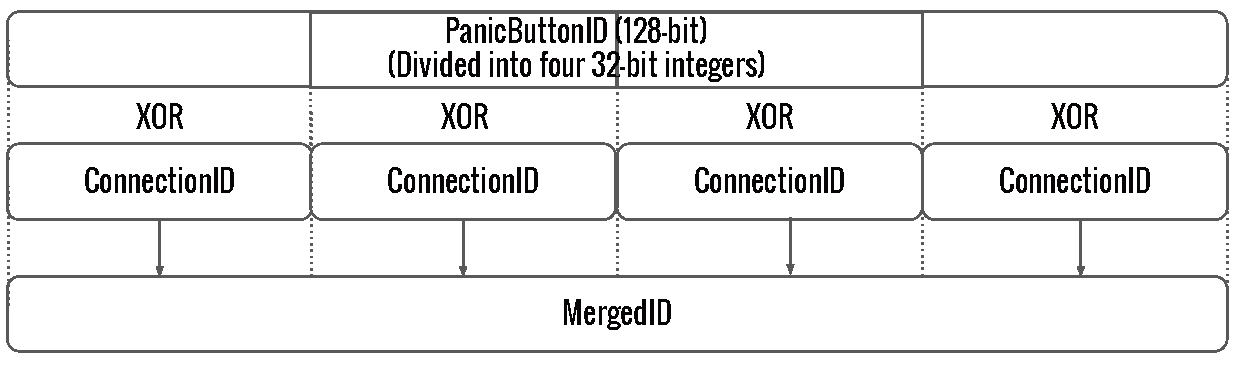
\includegraphics[scale=0.7]{merged_id.pdf}
\caption{Data flow for merging the connectionId and panicButtonID}
\label{fig:merged_id}
\end{figure}
\emph{MergedID} is encrypted to get \emph{cipherCode} by RSA algorithm using 256-bit public encryption key, which is stored in non-volatile memory of core-module.\\
The core-module will send Message Queuing Telemetry Transport (MQTT) message to \emph{``/gateway/validation"} topic in JavaScript Object Notation (JSON) format containing \emph{connectionID}, \emph{cipherCode}, \emph{date-time} and \emph{validationResult} fields.

\begin{figure}[H]
\centering
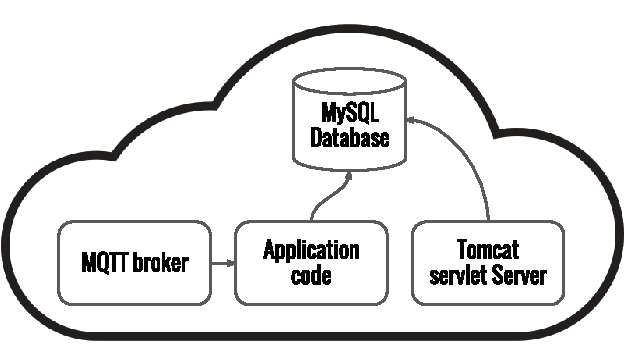
\includegraphics[]{server.pdf}
\caption{Overview of server running in the cloud}
\label{fig:server}
\end{figure}

\textbf{Server} is running a MQTT broker, a Tomcat servlet server, a MySQL database and application code to handle incoming MQTT messages as shown in figure~\ref{fig:server}.\\
Server is connected to the MySQL database, which has information of all the gateways \emph{PanicButton devices} and the vehicles. When a user's smartphone connects to server, it sends a unique random 32-bit \emph{connectionID}. When the \emph{PanicButton device} sends the validation results, it also sends the \emph{connectionID} to the server. The \emph{connectionID} is used to match the two connections (MQTT from \emph{PanicButton device} side and HTTP from smartphone side). Server waits for both connection to be established to synchronize the processing of the validation request.
 
The server holds the connection from user's smartphone until, it receives the same \emph{connectionId} in MQTT message in topic \emph{``/gateway/validation"} from \emph{PanicButton device}. Once the synchronization completes, the server decrypts the \emph{panicButtonID} using the secure private key stored in it. If the \emph{panicButtonID} exists in the database, the server sends the details to the smartphone or else it sends a NULL object to the smartphone. Server also sends validation results and date-time to the user's smartphone in JSON format. After sending the data, server closes the connection.\\


Next we will look into individual modules that gets validated.

\subsubsection{Microphone validation}
Microphone is one the most important module in the system. To Validate the microphone functionality, we are using a closed loop validation procedure as shown in figure~\ref{fig:mic_validation}.
\begin{figure}[H]
\centering
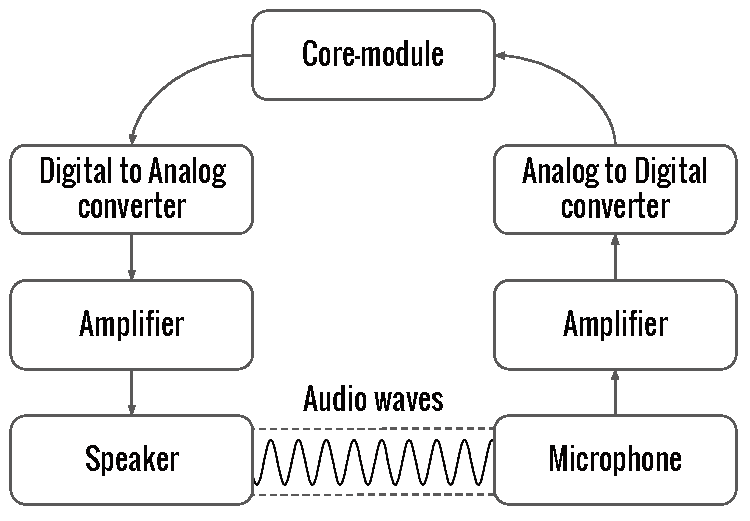
\includegraphics[scale=1]{mic_validation.pdf}
\caption{Microphone validation procedure}
\label{fig:mic_validation}
\end{figure}
Core-module generates a stream of pulsed single tone audio which corresponds to binary code of 10100101 and single tone frequency of 19 kHz as shown in figure~\ref{fig:waveform}.\\
\begin{figure}[H]
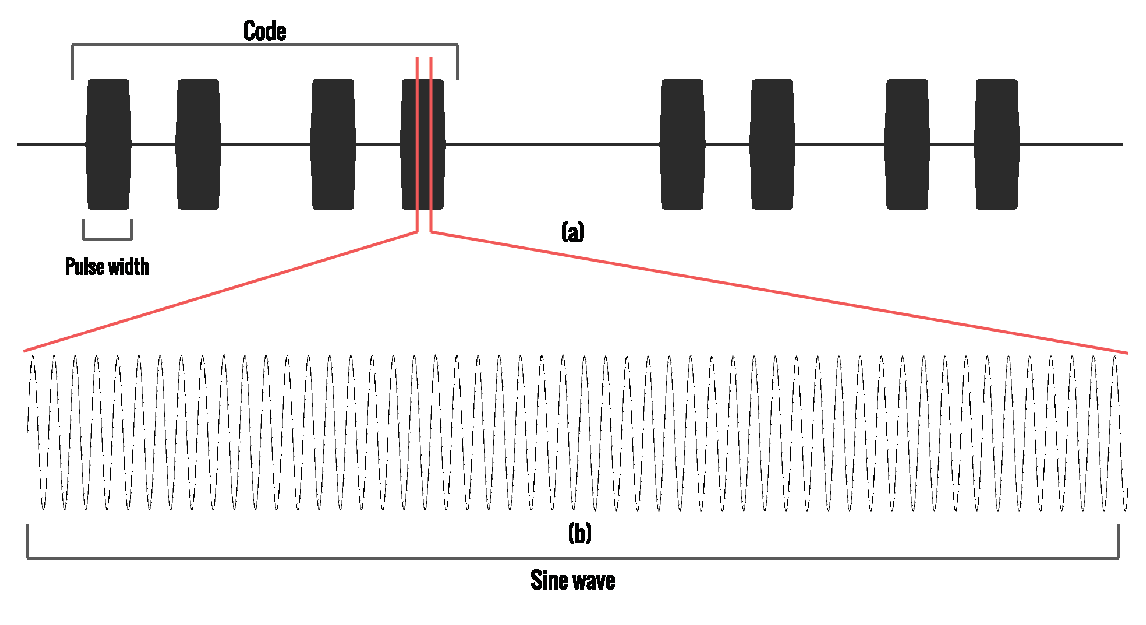
\includegraphics[width=\textwidth]{waveform.pdf}
\caption{Waveform of pulse single tone audio data (a) code sent via speaker (10100101) (b) sine wave of frequency 19000kHz}
\label{fig:waveform}
\end{figure}
\paragraph{Validation sequence\\}
For the validation of the microphone, we need two threads. First thread generates the audio stream and play it on the speaker and second thread analyses the audio stream received from the microphone to validate the microphone.\\
%subparagraph{Speaker Thread}
\textbf{Speaker thread} initializes the speaker to the default state and drains the existing audio date from the stream. Rise time of the waveform is not infinite, instead it rises slowly and linearly from zero to full amplitude in 3 ms. This helps in reducing high frequency harmonics. The audio data shown in figure~\ref{fig:waveform} is played through the speaker. After this operation, the speaker thread is suspended.\\
%\subparagraph{Microphone Thread}
\textbf{Microphone thread} initializes the microphone to the default state and flushes the existing audio data from the stream. Microphone waits for 441 samples to perform 441 point FFT. After calculating FFT, power around 19 kHz is calculated. The power calculated is then added to the time series queue of 50 samples, where the oldest power points are discarded. The \emph{correlation} is calculated for received time-series with the original data sent from the speaker. If the \emph{correlation} value exceeds the defined threshold then validation passes or else the process repeats until the timeout occurs. After the timeout it will retry microphone validation for two more times. If even after third try, the timeout occurs then validation is considered to be failed. The algorithm is explained in the flowchart shown in the figure~\ref{fig:mic_validation_flowchart}.
\begin{figure}[H]
\centering
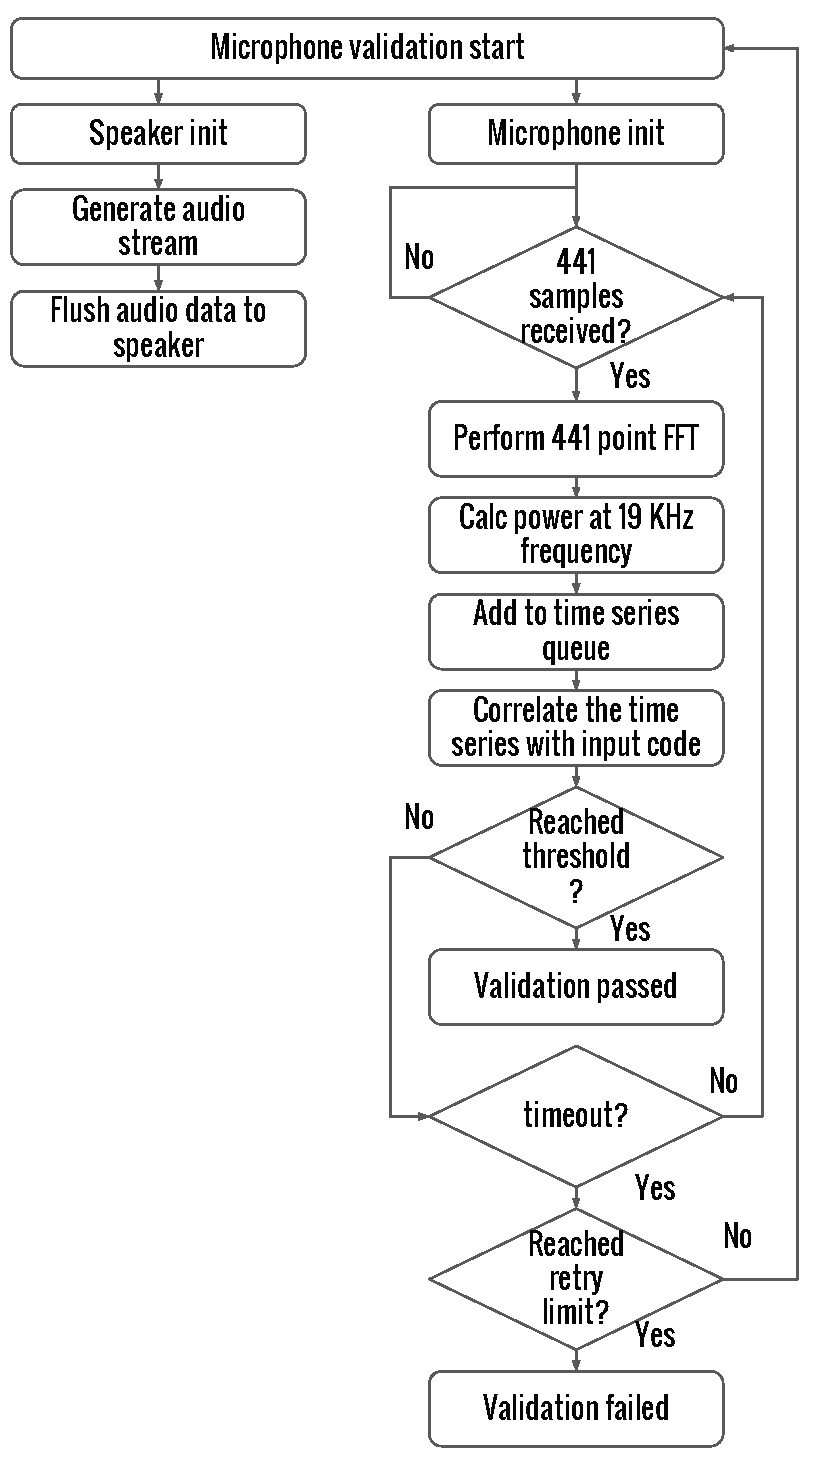
\includegraphics[width=0.7\textwidth]{mic_validation_flowchart.pdf}
\caption{Flow chart of microphone validation procedure}
\label{fig:mic_validation_flowchart}
\end{figure}
\subsubsection{Panic Button validation}
To validate the panic button, we emulate button press by shorting the pins of panic button by using the transistor as a switch, shown in figure~\ref{fig:p_button_a}. First the initial condition is tested for open. If the test passes then transistor pin is set to emulate button press. Second condition is tested for short. If the test passes then the validation succeeds. The transistor pin is reset which emulates button release. If any test fails then it will retry the procedure two more times. If even after third try, the test still fails then validation is considered to be failed. 
\begin{figure}[H]
\centering
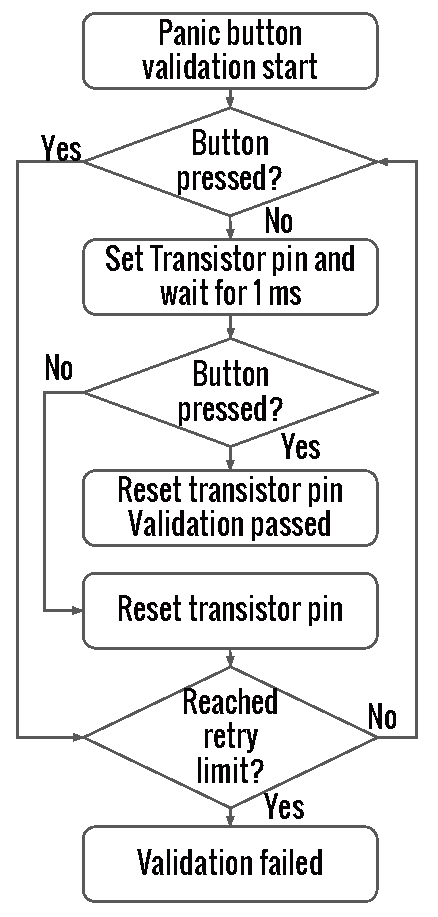
\includegraphics[scale=0.7]{panic_button_validation.pdf}
\caption{Flow chart of Panic Button Validation}
\label{fig:panic_button_validation}
\end{figure}
\subsubsection{Firmware validation}
Firmware validation is done after every soft/hard reset. To validate the firmware MD5 checksum is calculated for entire firmware and it is compared with the MD5 checksum stored in a non-volatile memory of core-module. If both match then firmware validation passes.
\subsubsection{Tamper detection}
We use an ultra low power MSP430 microcontroller for always-on tamper detection with its independent battery. Tamper is detected using a switch mounted inside the enclosure. MSP430 detects the tamper by detecting the change in logic level (from high level to low level) of this switch's pin. Once tamper is detected by MSP430 microcontroller, it permanently deletes the private key stored in the flash of the microcontroller. While servicing the device, lid opening will trigger the tamper detection event, but it can be suppressed by the server by the request of an authorized personal. The private key can be retrieved from the server and re-flashed into the flash of the microcontroller by an authorized personal.\\
The core-module regularly communicates with MSP430 and sends it a unique random number. MSP430 encrypts the number using TEA encryption algorithm (explained below) and sends it back. The core-module decrypts the number back from received data, on receiving mismatched numbers, tampering is notified to the server. The flow chart is shown in the figure~\ref{fig:tamper_proof}.
\begin{figure}[H]
\centering
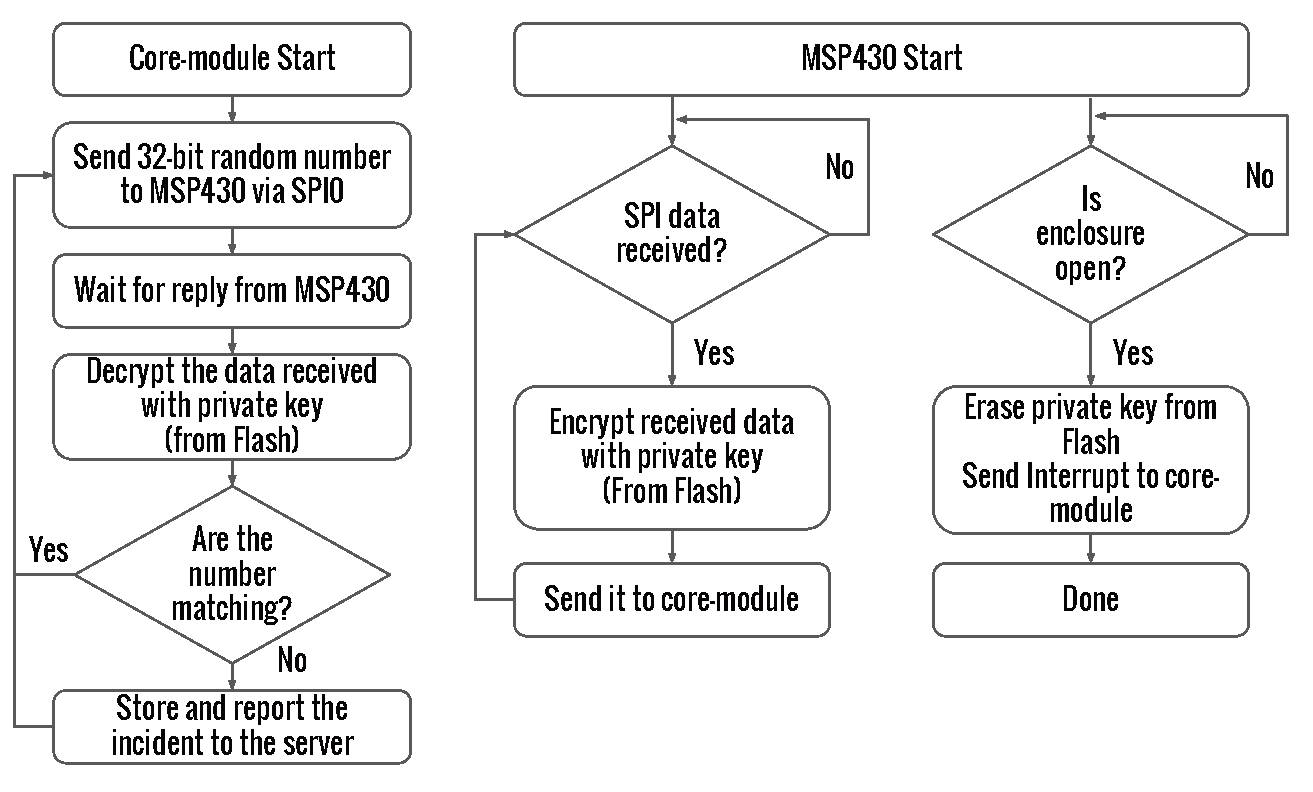
\includegraphics[scale=0.7]{tamper_proof.pdf}
\caption{Flow chart of tamper detection module}
\label{fig:tamper_proof}
\end{figure}
\paragraph{Encryption Algorithm\\}
The algorithm used is a modified version of Tiny Encryption Algorithm\cite{tea_paper}. Pseudo code of encrypt and decrypt subroutines are described in the figure~\ref{fig:msp_encryption}, where data variable is a 32-bit data to be encrypted and key is the 64-bit private key used to encrypt it.
\begin{figure}[H]
\centering
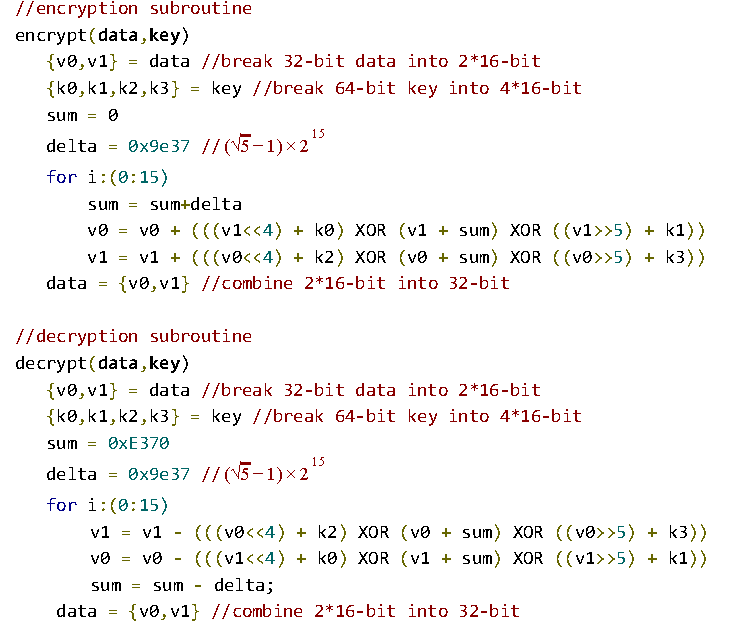
\includegraphics[width=\textwidth]{msp_encryption.pdf}
\caption{The pseudo code for the TEA encryption algorithm}
\label{fig:msp_encryption}
\end{figure}
The constants used are delta 0x9e37 ($(\sqrt{5}-1)*2^{15}$) and sum 0xE370 ((delta*16)*0xFFFF).
\subsection{Audio streaming module}
Streaming of realtime audio data with minimum latency is essential to the system for further analysis and storage as evidence in the hard-drives of the server.
Raw data is not suitable for streaming because of the sheer size of it. To compress the data, we have used Vorbis ogg\cite{vorbis_site} open-source patent free audio compression format, which is suitable the streaming and storage of audio data.\\
we used raw TCP socket to stream the audio data from the \emph{PanicButton device} to the server. We need a single stream of audio from the device, so the overhead of HTTP header is not required. The extra information required by the server is embedded inside the Vorbis ogg comments page. The data flow is shown in figure~\ref{fig:vorbis_stream}.
\begin{figure}[H]
\centering
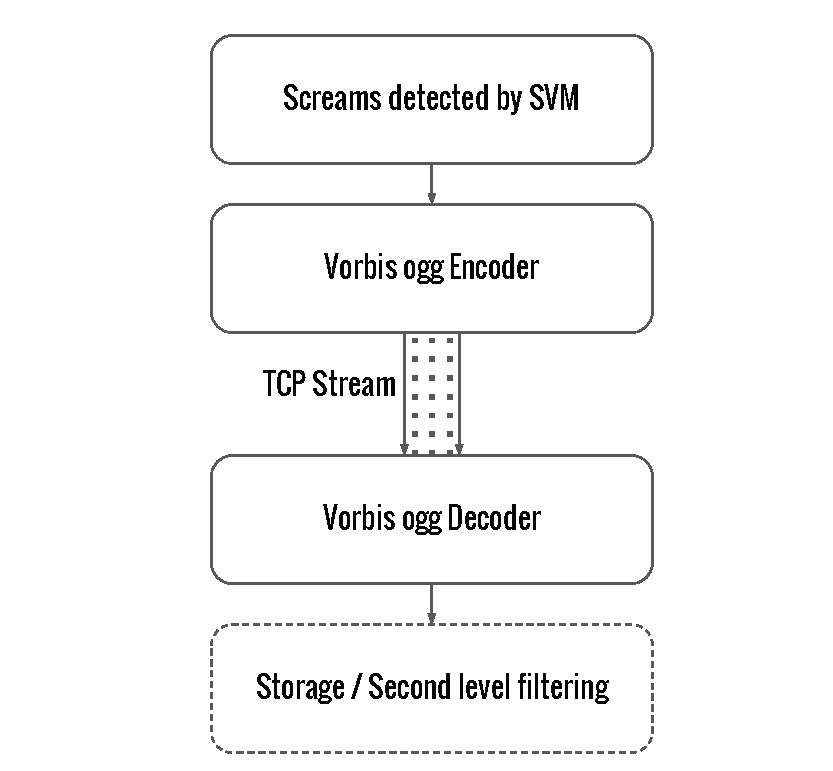
\includegraphics[scale=0.7]{vorbis_stream.pdf}
\caption{Data flow in streaming of audio data}
\label{fig:vorbis_stream}
\end{figure}
We used libvorbis, libogg and libvorbisenc open source libraries to encode and decode from the vorbis ogg format.

\subsection{Global positioning system module}
The NEO-6M module from ublox uses UART protocol for sending the GPS data to the host controller. It sends data in National Marine Electronics Association(NMEA) format. NMEA format consists of sentences, whose first word is called the data type, which defines the interpretation of the rest of the sentence. The NEO-6M module sends data with GPGGA and GPRMC data types. Core-module decodes the location and date-time information from the NMEA format.
\subsection{Panic button module}
The system needs realtime button response. To minimize the response latency, we used pin interrupt and timer combination  debouncing technique instead of using only timer based debouncing as shown in figure~\ref{fig:pin_interrupt}
\begin{figure}[H]
\centering
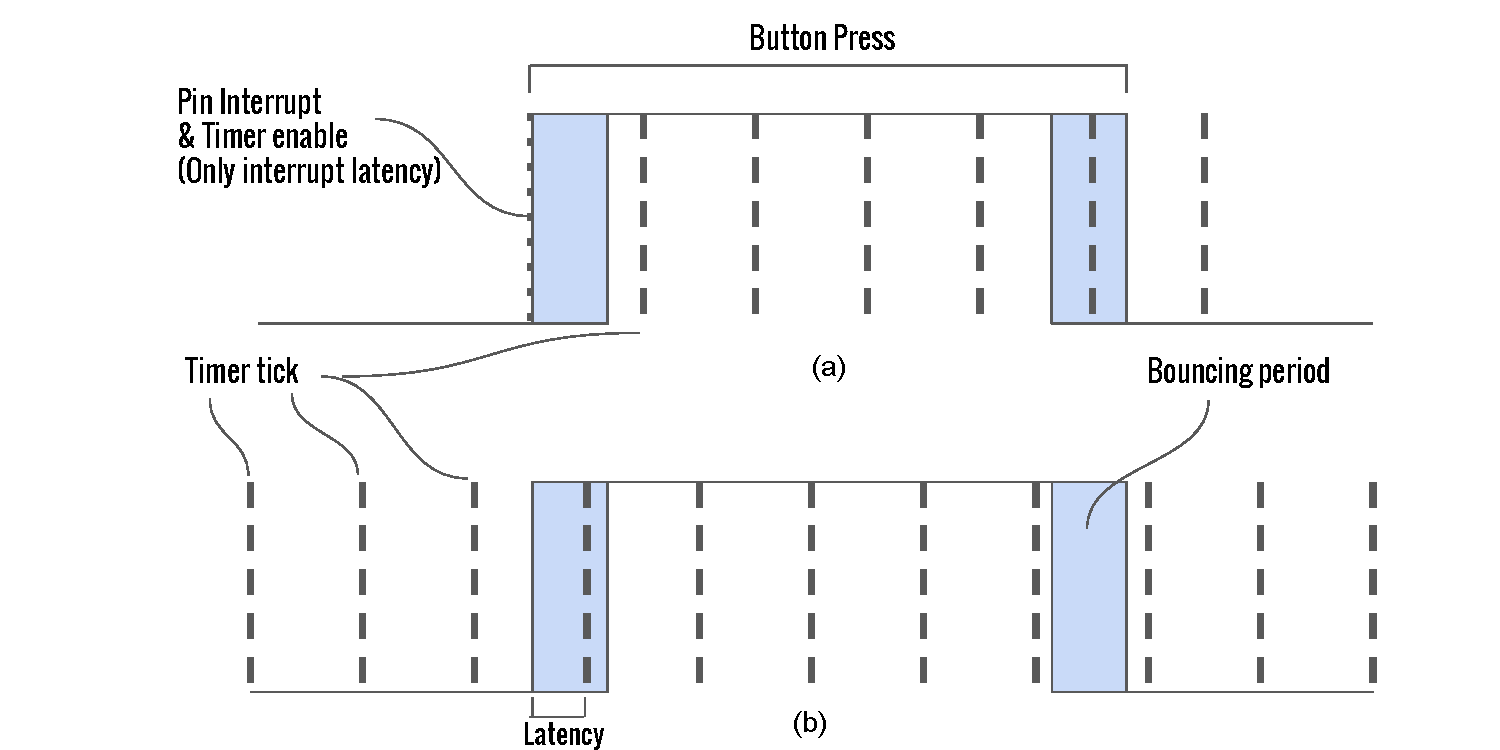
\includegraphics[width=\textwidth]{pin_interrupt.pdf}
\caption{Deboncing technique(a) Combination of pin interrupt and timer to reduce latency. (b) Only using timer interrupt.}
\label{fig:pin_interrupt}
\end{figure}
%TODO
The maximum period of debouncing is expected to be around 10ms\cite{debounce_paper}. We used timer tick period of 15 ms, which is greater than maximum debouncing period. In case (b) maximum latency is 15 ms and in case (a) maximum latency is of  only six cycles (0.375 us) for pin interrupt. Hence we opted for method (a).

\subsection{Audio-based trigger module}
As described in study section, we decided to use Support Vector Machine (SVM) as underlying machine learning algorithm and Mel-Frequency Cepstral Coefficients (MFCC) as feature set for this algorithm  to detect scream. Let's have a look at feature extraction procedure used in this project.
\subsubsection{Feature Extraction}
Mel-Frequency Cepstral Coefficients (MFCC), which acts as feature set, are extracted from live stream of input audio. Figure~\ref{fig:Featureextraction} depicts the Feature extraction procedure.

\begin{figure}[H]
\centering
\def\svgwidth{\textwidth}
\input{feat.pdf_tex}
\caption{Feature extraction process}
\label{fig:Featureextraction}
\end{figure}

Every second audio data is fetched from sound card and dumped into an input fifo, this 1 second of audio data is then appended with previous 0.98 second (0.98 second is multiple of 30 ms, which is the window size used in the FFT operation) of audio data. MFCC features are extracted for this composite audio clip.

MFCC are computed by first chopping the audio signal into tiny overlapping segments, these segments are multiplied with a window function like Hamming window; Fourier transform is computed over this windowed audio segment. The power spectrum is wrapped according to Mel-scale to adapt the frequency resolution of human ear. This spectrum is then segmented into number of critical bands using a triangular filter bank; Inverse Discrete Cosine Transform (DCT) applied to the logarithm of filter bank's outputs result in MFCC vector.

We obtain super feature vector of R\textsuperscript{24} for each 1.98 sec of audio data. This super feature vector is obtained by taking column mean and standard deviation of 169 x 12 matrix, which was obtained by extracting MFCC(ignoring 0\textsuperscript{th} MFC coefficient) for audio data of 1.98 sec. Once features are extracted, they are used for training the SVM.  

\subsubsection{Training of SVM}
\paragraph{Training-\\}

Like all machine learning algorithms, we need to train our SVM using a labeled data set. Labeled data set contains data that is painstakingly labeled by a human, classifying whether a particular 1.98 second clip is a scream. Clip is labeled 1 for a scream and -1 for not a scream. Figure~\ref{fig:train} depicts the training process.
 
\begin{figure}[H]
\centering
\def\svgwidth{\textwidth}
\input{train.pdf_tex}
\caption{Training process of the SVM}
\label{fig:train}
\end{figure} 
Support Vector Machine (SVM) uses a kernel to transform data into higher dimension space and finds a linear separating hyper plane with maximal margin in this higher dimensional space. We are using radial basis function (RBF) as kernel, due to its ability to model complex data patterns. RBF kernel \(K(x_i,x_j)\)
is defined as- \[K(x_i,x_j)=exp(-\gamma\parallel(x_i-x_j)\parallel^2), \gamma>0.\]
For training SVM that uses RBF kernel, we need to specify values of two parameters -
\begin{enumerate}
 \item C (penalty factor used in cost function) and 
 \item \(\gamma\) ( variance of the RBF kernel).
\end{enumerate}
 We used following steps to get optimum value of C and \(\gamma\) and use them for the training-
\begin{enumerate}
\item Arrange data in proper format i.e., [data,label],
\item Randomize the data in cross-validation set,
\item Consider the RBF kernel \(K(x,y)=e^{(-\gamma\parallel(x_i-x_j)\parallel^2)}\),
\item Use cross-validation set to find the best values for parameters C and \(\gamma\),
\item Use these values of C and \(\gamma\), to train the SVM from training data set and
\item test.
\end{enumerate}

We will dwell into details of these steps in section \ref{sssec:FindCandgamma}, first lets have a look at data set used in this project. 

\paragraph{Data set-\\}

Data set used in this project is called IIITD Urban Environment Context database (IUEC)\cite{paper10}. It contains audio clips from following environmental contexts-
\begin{enumerate}
\item Conversation (narrations)
\item Human gathering (clubs and meetings)
\item Indoors (indoor sounds)
\item machinery (fan, shaver, laptop-fan, exhaust, oven, mixer, washing machine and vacuum cleaner)
\item Multimedia (movie audio and TV audio)
\item Outdoors (bus stand, road traffic, market, temple, rickshaw, rain, metro and playground)
\item distress (scream and crying sounds)
\end{enumerate}

Table~\ref{tab:quandata} quantifies the content of this dataset.
\begin{table}[H]
\begin{center}
\begin{tabular}{ |c|c| } 
 \hline
 \textbf{Context} & \textbf{Samples of 2 sec} \\ 
 \hline
 \hline
 Conversation & 623 \\
 \hline 
 Human gathering & 1621 \\ 
 \hline
 Indoors & 4169 \\
 \hline
 Machinery & 3548 \\
 \hline
 Multimedia & 3698 \\
 \hline
 Outdoors & 5142 \\
 \hline
 Scream & 464 \\
 \hline
 \hline
 \textbf{Total} & \textbf{19265= 10 Hrs 42 Mins}\\
 \hline
\end{tabular}
\end{center}
\caption{IUEC Data set details} \label{tab:quandata}
\end{table}

Apart from this data set, we collected data using the \emph{PanicButton device} prototype. Table~\ref{tab:quandata2} quantifies its content.
\begin{table}[H]
\begin{center}
\begin{tabular}{ |c|c| } 
 \hline
 \textbf{Context} & \textbf{Samples of 2 sec} \\ 
 \hline
 \hline
 Conversation & 1144 \\ 
 \hline
 Multimedia & 1828 \\
 \hline
 Outdoors & 2623 \\
 \hline
 Scream & 464 \\
 \hline
 \hline
 \textbf{Total} & \textbf{6059= 3 Hrs 22 Mins}\\
 \hline
\end{tabular}
\end{center}
\caption{Details of data collected from panic button prototype} \label{tab:quandata2}
\end{table}

Scream samples were obtained by re-recording scream data available in IUEC data set. We combined this two data sets to get a composite data set, whose content is quantified in Table~\ref{tab:quandata3}
\begin{table}[H]
\begin{center}
\begin{tabular}{ |c|c| } 
 \hline
 \textbf{Context} & \textbf{Samples of 2 sec} \\ 
 \hline
 \hline
 Conversation & 1767 \\
 \hline 
 Human gathering & 1621 \\ 
 \hline
 Indoors & 4169 \\
 \hline
 Machinery & 3548 \\
 \hline
 Multimedia & 5526 \\
 \hline
 Outdoors & 7765 \\
 \hline
 Scream & 928 (3.6\% of complete data set)\\
 \hline
 \hline
 \textbf{Total} & \textbf{25324= 14 Hrs 4 Mins}\\
 \hline
\end{tabular}
\end{center}
\caption{Composite Data set details} \label{tab:quandata3}
\end{table}

This complete data set gets divided into two equal parts called training data set and cross-validation data set. Training data set is used for training the SVM and cross-validation dataset is used for tuning the SVM. Our data set is highly skewed i.e., scream samples constitutes only 3.6\% of the complete data set. This makes benchmarking of trained SVMs non-conventional. Section~\ref{sssec:FindCandgamma} addresses this problem in detail.

Finally, a test clip of 22 minutes was created to quantify performance of the trained SVM. This 22 minute clip was carefully designed to cover audio samples from every context. Obtained results are mentioned in Section~\ref{sssec:performanceSVM}.

\subsubsection{Finding C and gamma} 
\label{sssec:FindCandgamma}
To find the optimum value of C and \(\gamma\), we performed grid search for these parameters on cross-validation data set. Five fold cross-validation data set (4 part for training and 1 part for testing in circular fashion for a particular combination of C and \(\gamma\)) is used. Figure~\ref{fig:CVflowchart} shows the process of finding optimum C and \(\gamma\).

\begin{figure}[H]
\centering
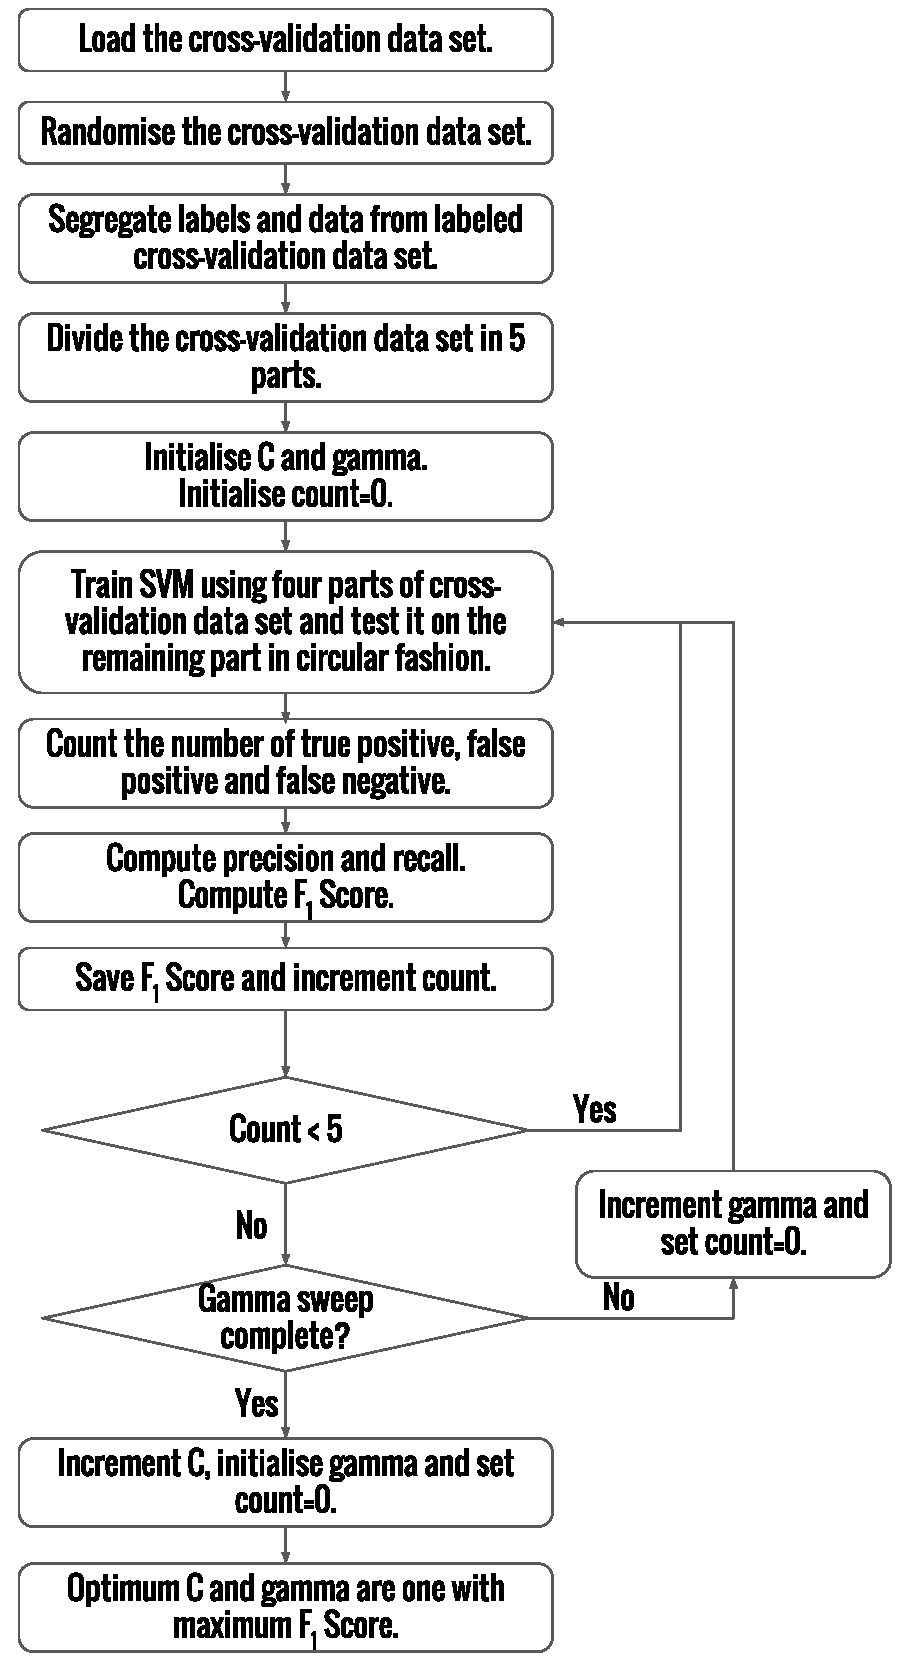
\includegraphics[scale=0.85]{CVflowchart.pdf}
\caption{Cross-validation process for obtaining optimum C and gamma}
\label{fig:CVflowchart}
\end{figure}

Method shown in figure~\ref{fig:CVflowchart} is a brute force method to find optimum value of C and \(\gamma\). We use \(F_1\) score as figure of merit (FOM); Accuracy can't be used as FOM due to skewed nature of data set.

\(F_1\) score is computed using precision (prec) and recall (rec):\[F_1=\dfrac{2 . prec . rec}{prec+rec},\] We can compute precision and recall by: \[prec=\dfrac{t_p}{t_p+f_p}\]
\[rec=\dfrac{t_p}{t_p+f_n}\]
where
\begin{itemize}
\item \(t_p\) is the number of true positives: the ground truth label says it's a scream and our algorithm correctly classified it as a scream.
\item \(f_p\) is the number of false positives: the ground truth label says it's \textbf{not} a scream, but our algorithm incorrectly classified it as a scream.
\item \(f_n\) is the number of false negatives: the ground truth label says it's a scream, but our algorithm incorrectly classified it as \textbf{not} a scream.
\end{itemize}

In any automated alarm system, ideally we should have zero false negative, practically it should be as small as possible. Following figure show us the $F_1$ score obtained by performing grid search for the parameters C and \(\gamma\) on the cross-validation set.
\begin{figure}[H]
\centering
\def\svgwidth{\textwidth}
\input{F1score.pdf_tex}
\caption{F1 score obtained from grid search for C and gamma on CV set}
\label{fig:f1score}
\end{figure} 

Once we have the value of C and \(\gamma\), we can use that value to train our SVM. This process of first obtaining appropriate value of C and \(\gamma\) and then training the final SVM, helps us in avoiding machine learning traps like over-fitting and under-fitting.
Performance of the trained SVM is quantified in section~\ref{sssec:performanceSVM}, besides figure~\ref{fig:f1score} also quantifies the performance of best SVM, over the five fold cross-validation set.

\subsubsection{Performance of the SVM}
\label{sssec:performanceSVM}

We performed benchmarking using a 22 minute test set, this test set contains 24 screams of different lengths and strengths. We were able to detect 23 screams with 1 false negative and 3 false positive, giving us accuracy of \textbf{95.8\%} and \(F_1\) score of \textbf{0.92} with latency of 1.480 ms.


%Based on the input and output stimuli classification of each %software
%module or sub-module, perform the algorithm design which includes,
%\begin{itemize}
%\item numeric format for the application in case of embedded %software (floating
%point or fixed point and positioning of the virtual binary point)
%\item normalising and scaling constants
%\item module inputs and type
%\item module output and type
%\item module constants
%\item global constants
%\item referred subroutines
%\item algorithm in pseudocode
%\end{itemize}
%NOTE: \emph{include as many sections/sub-sections as there are %software
%modules/sub-modules and repeat the above for every software module
%and sub-module}.


\section{Industrial design}
\subsection{Module design}
Connected panic button's industrial design is divided as follows-
\begin{itemize}
\item Design of top panel,
\item Design of panic button,
\item Design for the tamper detection circuit and,
\item Design of the base.
\end{itemize}

\subsubsection{Design of top panel}
Top panel of the \emph{PanicButton device} acts as host to emergency button, speaker and microphone. The panic button's stem passes through the center of the front panel. Just beside the grove for passing the stem of emergency button, is a whole of radius 4 cm, which acts as speaker housing. One more hole of radius 0.5 cm is kept besides the house of speaker for mounting microphone. 

Speaker and microphone are assembled in a manner that the sound produced from speaker gets directly coupled to the microphone from outside the enclosure. A cap was designed around the speaker, to minimize the coupling of sound from inside the enclosure. Bottom part of the panic button plays an important role in this coupling of audio and is discussed in section~\ref{sssec:designemergency}. Figure~\ref{fig:toptop} shows the top view of the top panel and figure~\ref{fig:bottomtop} shows the bottom view of the top panel.

\begin{figure}[H]
\centering
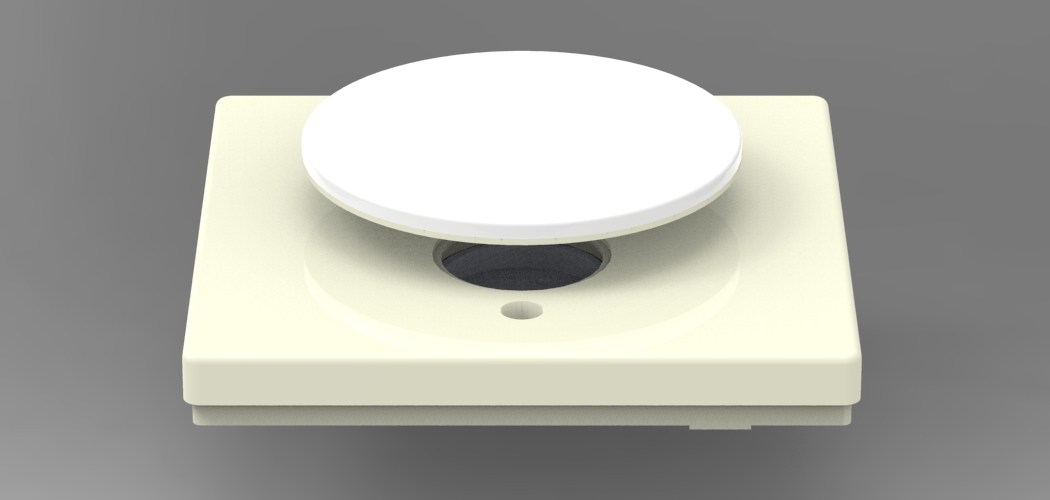
\includegraphics[width=\textwidth]{untitled_231.jpg}
\caption{Top view of the top panel of the \emph{PanicButton device}}
\label{fig:toptop}
\end{figure}

\begin{figure}[H]
\centering
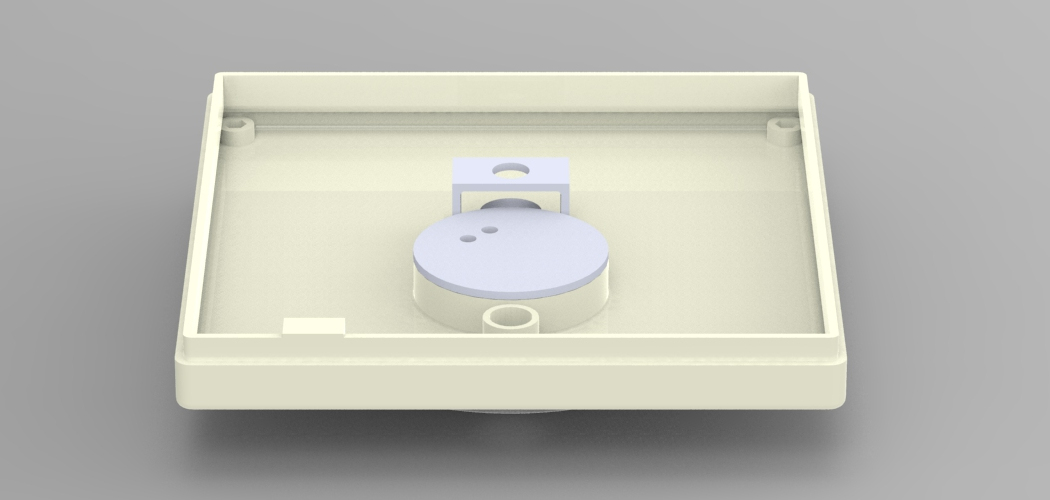
\includegraphics[width=\textwidth]{untitled_241.jpg}
\caption{Bottom view of the top panel of the \emph{PanicButton device}}
\label{fig:bottomtop}
\end{figure}

\subsubsection{Design of panic button}
\label{sssec:designemergency}
To make panic button easily accessible at all times, we took care of following two things.
\begin{itemize}
\item Area of the panic button equals the average area of a adult human's palm and
\item Back-light is added to the panic button to make sure that it is easily visible in the night. 
\end{itemize}

An important part of the emergency button design is to make sure that the button does not cover the microphone, while completely covering the speaker; Proper placement of these three component and size of button can take care of this.

Bottom part of the panic button acts as a reflector for sound produced by the speaker. For efficient performance of microphone validation procedure, it is important that the waves produced by the speaker are channeled to the microphone. To accomplish this task, bottom part of panic button was given a concave shape such that microphone lies at the focal point of the concave surface.

Stem of the emergency button was made hollow to pass wires for the back-light mounted inside the emergency button.
 
\subsubsection{Design for the tamper detection circuit}
Tamper detection circuit takes the input from a push button, that gets pushed once the top panel is mounted on the base of the enclosure. We designed a projection coming out of the wall to support the mounting of the switch. Figure~\ref{fig:tamper_detection_switch} shows the placement and shape of the projection.

\begin{figure}[H]
\centering
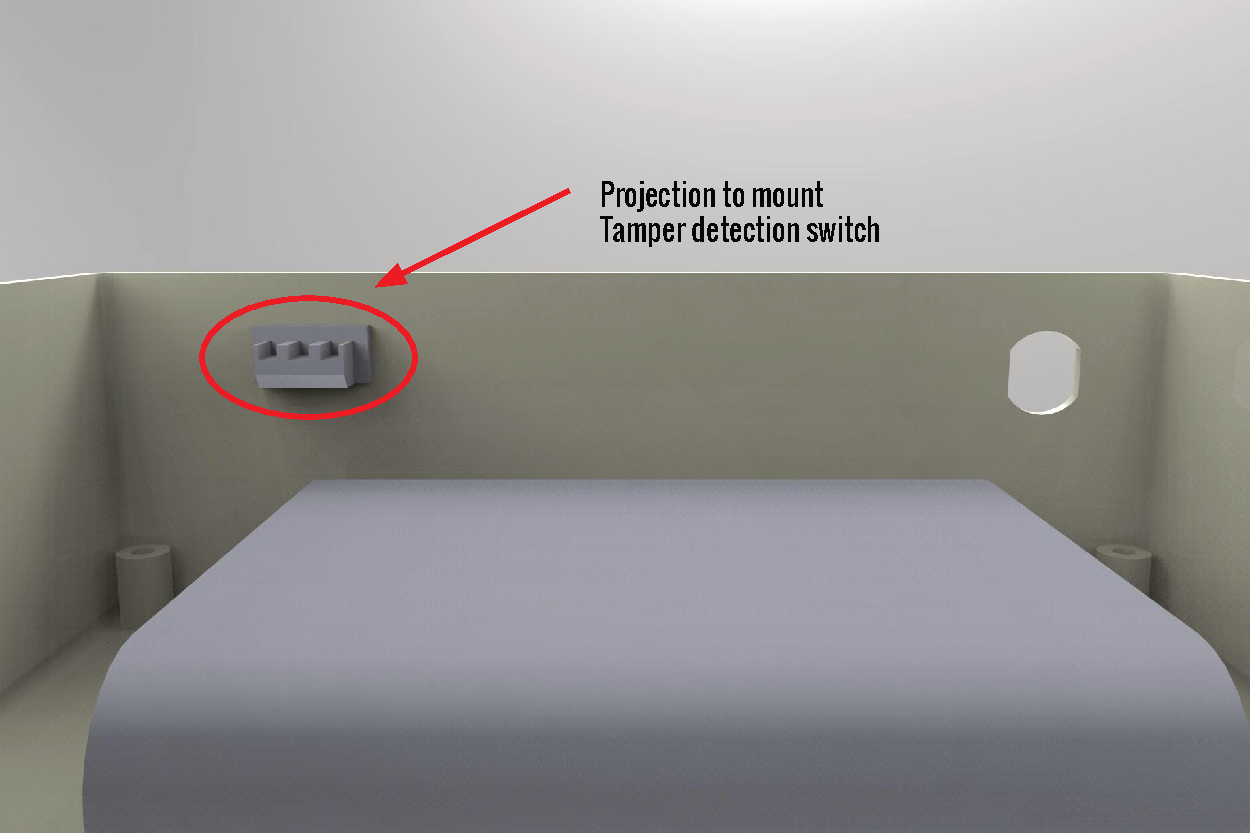
\includegraphics[width=\textwidth]{tamper_detection_switch}
\caption{The projection to mount the tamper detection switch}
\label{fig:tamper_detection_switch}
\end{figure}  

\subsubsection{Design of the base}
The base of the enclosure act as the host for all components residing inside the \emph{PanicButton device}. We placed 4 mounting holes for the raspberry pi and 4 m3 screw holes for bringing top and base together.

\subsection{Putting modules together}
\label{sec:desIndust}
Figure~\ref{fig:des_views} shows the \emph{PanicButton device}, once all modules are brought together and figure~\ref{fig:exploded_views} shows the exploded view of the \emph{PanicButton device}.  
\begin{figure}[H]
\begin{subfigure}{.5\textwidth}
  \centering
  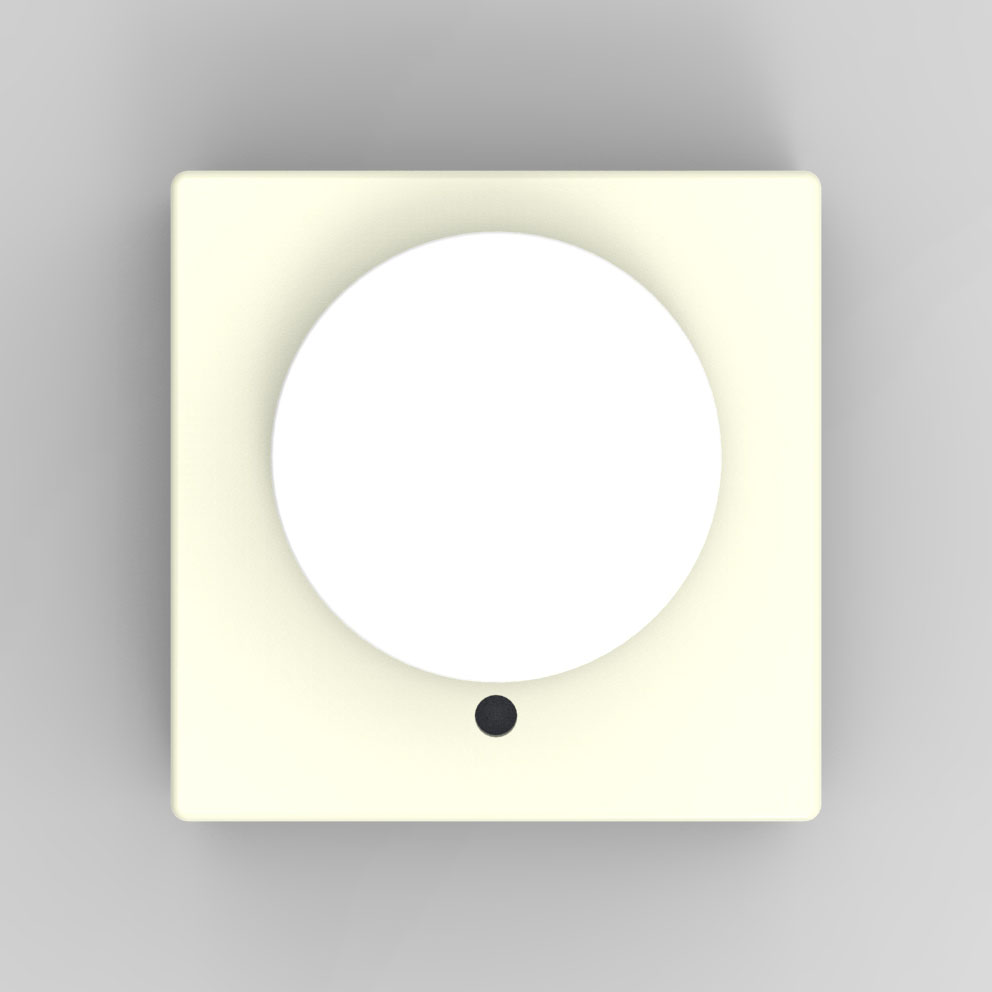
\includegraphics[width=.9\linewidth]{des_top_view}
  \caption{Top view}
  \label{fig:des_top_view}
\end{subfigure}%
\begin{subfigure}{.5\textwidth}
  \centering
  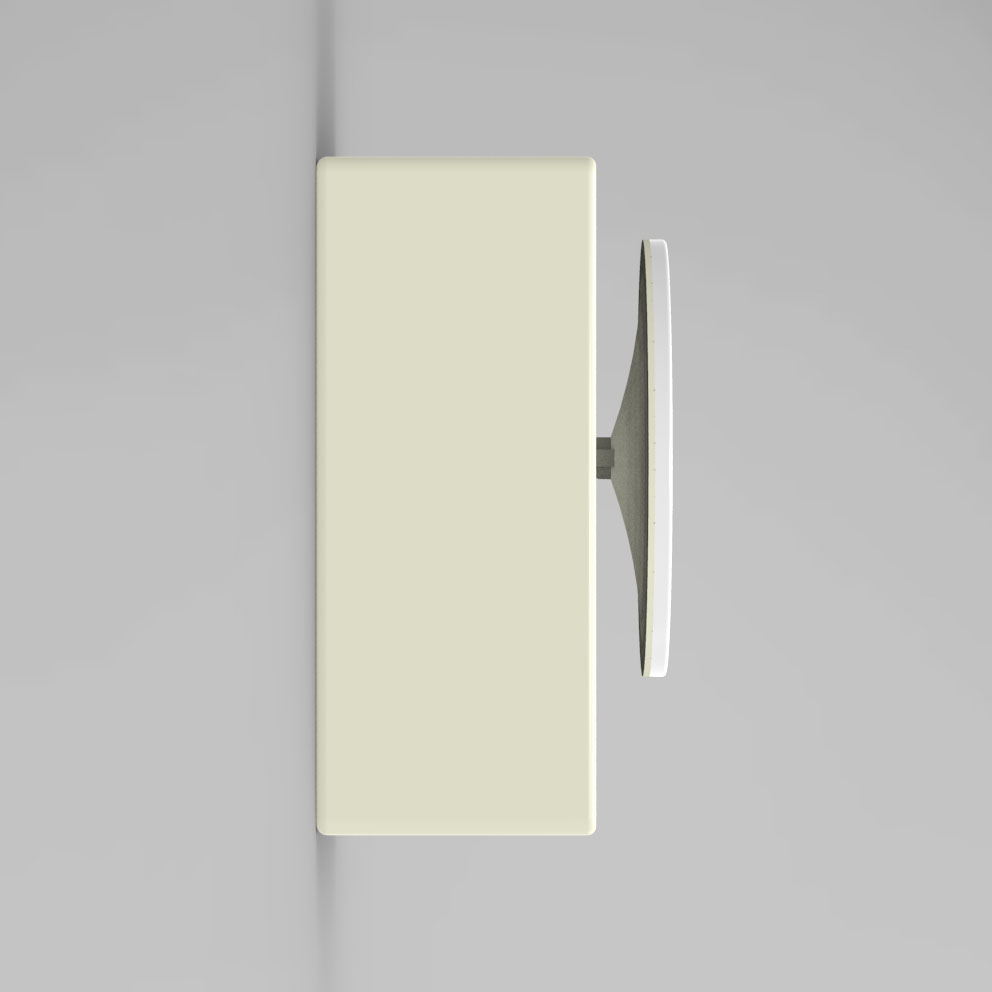
\includegraphics[width=.9\linewidth]{des_side_view}
  \caption{Side view}
  \label{fig:des_side_view}
\end{subfigure}
\begin{subfigure}{.5\textwidth}
  \centering
  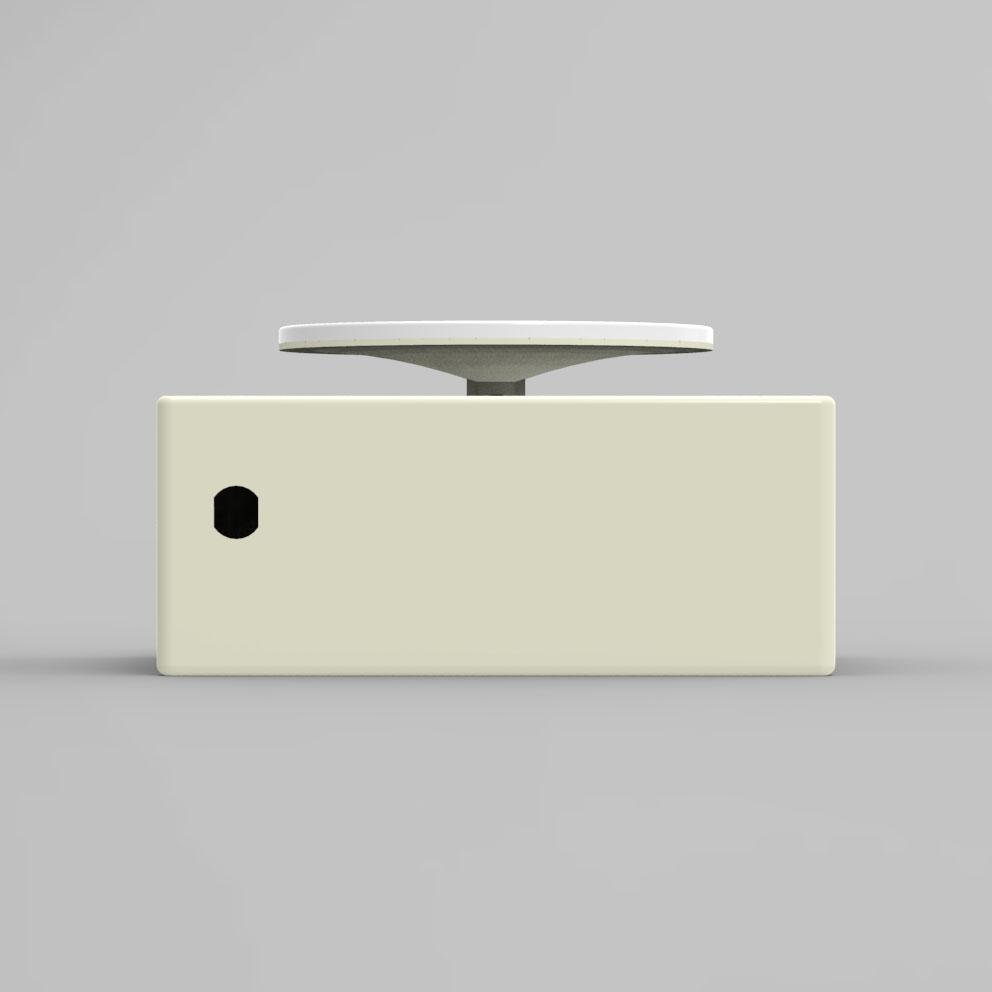
\includegraphics[width=.9\linewidth]{des_front_view}
  \caption{Front view}
  \label{fig:des_side_view2}
\end{subfigure}%
\begin{subfigure}{.5\textwidth}
  \centering
  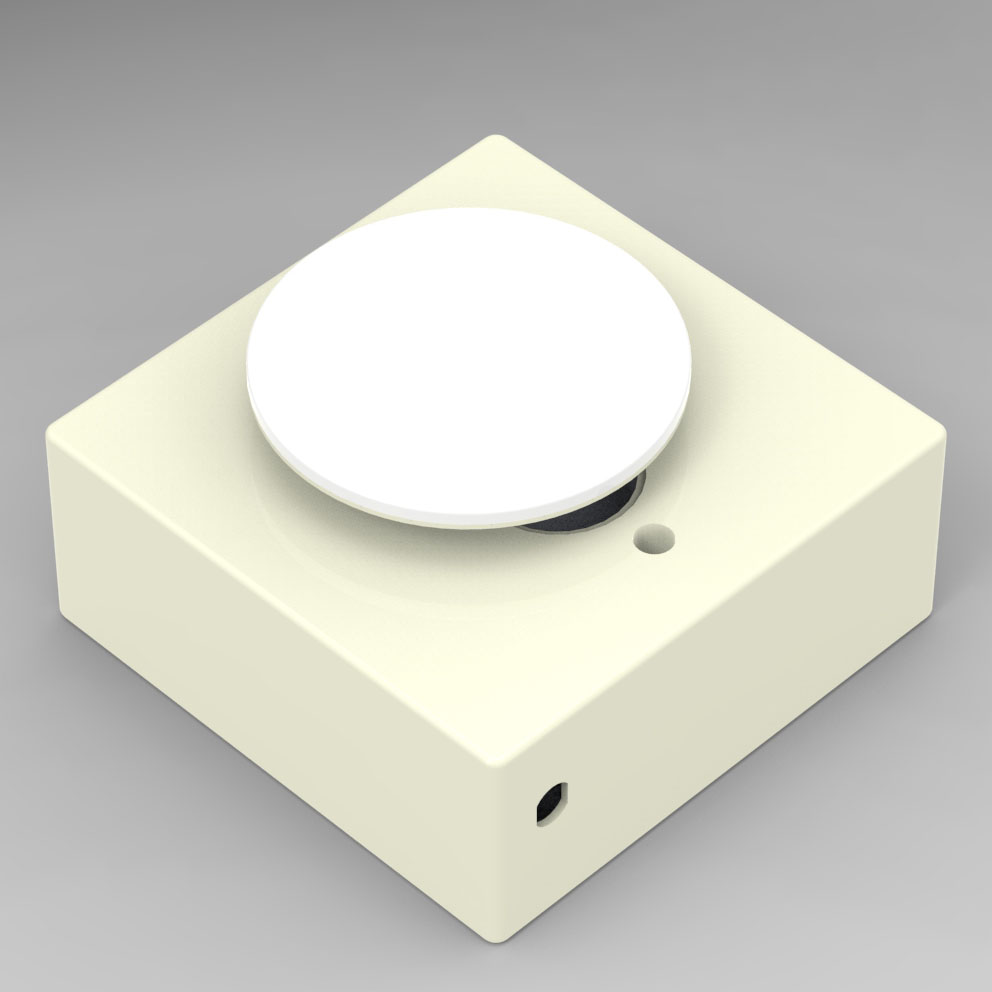
\includegraphics[width=.9\linewidth]{des_iso_view}
  \caption{Isometric view}
  \label{fig:des_iso_view}
\end{subfigure}
\caption{Top, side, front and isometric views of the enclosure}
\label{fig:des_views}
\end{figure}

\begin{figure}[H]
  \centering
  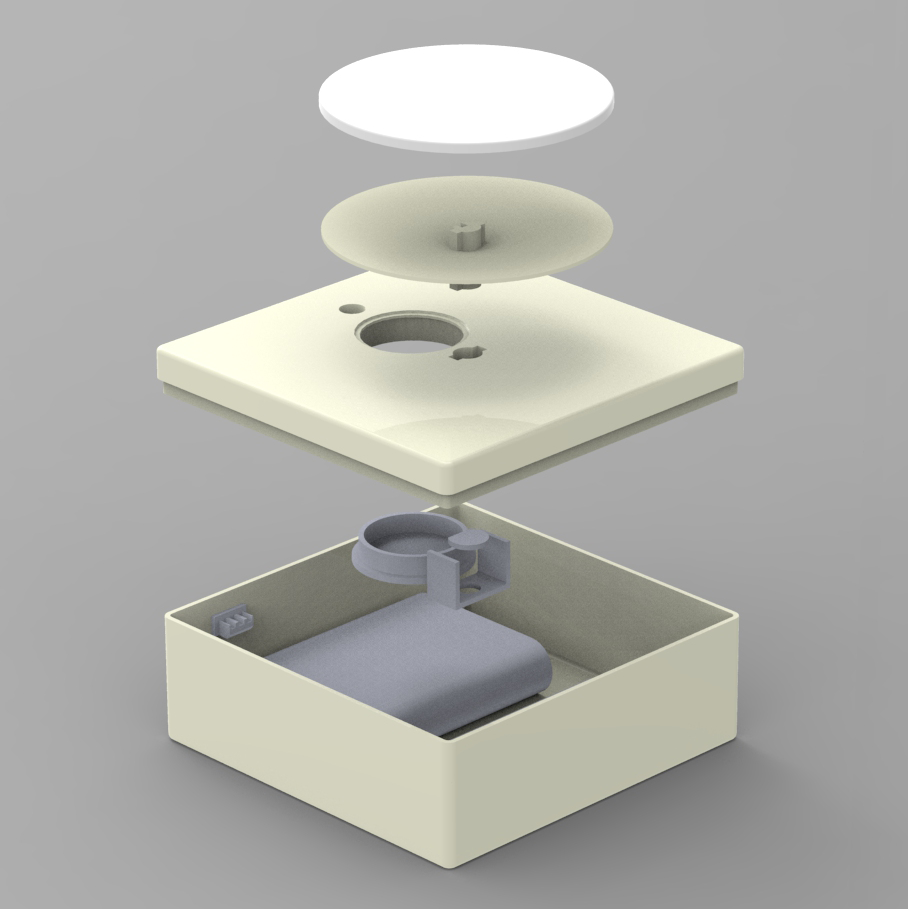
\includegraphics[width=.8\linewidth]{exploded_iso}
\caption{Exploded views of the enclosure}
\label{fig:exploded_views}
\end{figure}

%The section should include the following
%\begin{itemize}
%\item enclosure design (considering function, ergonomics and aesthetic)
%\item front panel design
%\item back panel design
%\item inter-module wiring and interconnection routing
%\item issues and considerations related to user interactions
%\item issues related to maintainability
%\item exploded view\end{itemize}

